\documentclass[12pt]{article}

\usepackage{verbatim}
\usepackage{listings}
\usepackage{color}
\usepackage{graphicx}
\usepackage{amsmath}


%%
\title{Xylophone Project}

\author{Fabien Le Mentec\\
\small \texttt{texane@gmail.com}
}

\date{}

\begin{document}
\maketitle

%%
\newpage
\begin{abstract}
This document describes the building of an electromechanical xylophone.
Copper
\end{abstract}

%%
\newpage
\section{Introduction}


%%
\newpage
\section{Pipes}

\subsection{Materials}
\paragraph{} We use copper pipes as vibrating elements. The main reasons being
copper is simple to work with, easily found in local stores and cheap.
\begin{center}
  \begin{tabular}{c|c}
    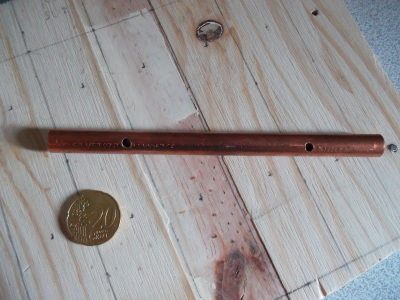
\includegraphics[keepaspectratio=true, width=40mm]{../pics/copper_pipe/full_scaled.jpg} &
    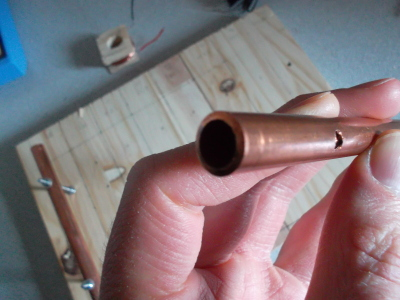
\includegraphics[keepaspectratio=true, width=40mm]{../pics/copper_pipe/inner_scaled.jpg}
  \end{tabular}
\end{center}

\subsection{Computing pipe length}
\paragraph{} The length depends on 3 factors:
\begin{itemize}
  \item the required frequency,
  \item the vibrating element shape,
  \item the sound propagation speed in the medium.
\end{itemize}
According to [wiki\_acous\_reson], the formula for a cylinder is:
\begin{center}
  \framebox[3in][c]{$ f = \frac{nv}{2(l + 0.8d)} $}
\end{center}
where:
\begin{itemize}
  \item $f$ the frequency in $hz$,
  \item $n$ an integer (1, 2, 3 ...),
  \item $v$ the speed of sound in medium in $ms^{-1}$,
  \item $l$ the length in $mm$,
  \item $d$ the cylinder diameter in $mm$.
\end{itemize}
However, we found an apparently better formula in [tamhigh\_xylo]
which accounts for the pipe radius of gyration. The nth transveral
frequency is given by:
\begin{center}
  \framebox[3in][c]{$ f_{n} = \frac{\pi v k}{8l^2} m^2 $}
\end{center}
where:
\begin{itemize}
  \item $f_{n}$ the frequency in $hz$,
  \item $v$ the speed of sound in medium in $ms^{-1}$,
  \item $k$ the gyration of radius,
  \item $l$ the length in $mm$,
  \item $m$ a value such that:
    \begin{itemize}
      \item $m = 3.0112$ when $n = 1$,
      \item $m = 5$ when $n = 2$,
      \item $m = 7$ when $n = 3$,
      \item $m = 2(n + 1)$ otherwise.
    \end{itemize}
\end{itemize}
For a tube, the radius of gyration is:
\begin{center}
  \framebox[3in][c]{$ k = \frac{1}{2} \sqrt{R^2 + r^2} $}
\end{center}
where:
\begin{itemize}
  \item $R$ the outter radius in $mm$.
  \item $r$ the inner radius in $mm$,
\end{itemize}
The copper sound propagation speed is:
\begin{center}
  \framebox[3in][c]{$3700 ms^{-1}$}
\end{center}

\paragraph{} Since we want the whole device small, we keep the pipe as short
as possible. However, we want to build it using relatively inaccurate
drilling and cutting tools. Thus, we ended up choosing the 8th frequency mode
(ie. the DO note frequency is 2093 hz), which results in the following table:
\begin{center}
  \begin{tabular}{|c|c|c|c|}
    \hline
    \textit{frequency (hz)} &
    \textit{length (mm)} &
    \textit{first node (mm)} &
    \textit{second node (mm)} \\
    \hline
    2093.000000 & 0.141960 & 0.031799 & 0.110161 \\
    \hline
    2349.313067 & 0.133993 & 0.030014 & 0.103978 \\
    \hline
    2637.014757 & 0.126472 & 0.028330 & 0.098142 \\
    \hline
    2793.819815 & 0.122872 & 0.027523 & 0.095349 \\
    \hline
    3135.956712 & 0.115976 & 0.025979 & 0.089997 \\
    \hline
    3519.992394 & 0.109466 & 0.024520 & 0.084946 \\
    \hline
    3951.057873 & 0.103322 & 0.023144 & 0.080178 \\
    \hline
    4186.010000 & 0.100381 & 0.022485 & 0.077896 \\
    \hline
\end{tabular}
\end{center}

\subsection{Cutting the pipes}
\paragraph{} The easiest and most accurate way to cut the pipe is by using a pipe cutter:
\begin{center}
  \begin{tabular}{c}
    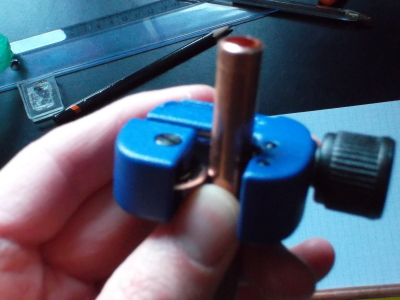
\includegraphics[keepaspectratio=true, width=40mm]{../pics/tools/pipe_cutter_scaled.jpg}
    \\
    \smallskip
    \tiny{\textit{pipe cutter}}
  \end{tabular}
\end{center}
We found experimentally that we must add roughly 1.5mm to the previously computed length.
This is due to the transversal holes and the vibration effects when the pipe is finally
mounted. By the way, it is always better to have a longuer pipe, since we can reduce it
with a lime for tuning until it reaches the correct frequency.

\subsection{Drilling the pipes}
TODO

\subsection{Checking the frequence}
TODO
\begin{itemize}
  \item video of xanalyzer -rate 16000
  \item recording audio files
\end{itemize}

%%
\newpage
\section{Assembling}

\subsection{Drilling the base}
\paragraph{} Drill the pipe transversal holes before drilling the base holes. Once this is
done, mark the base to prepare the drilling. It helps correcting small errors made while
percing  he pipe holes.

\subsection{Mounting the pipes}
\begin{center}
  \begin{tabular}{c|c}
    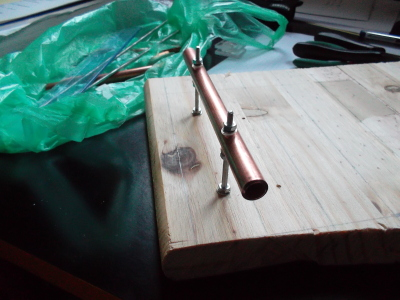
\includegraphics[keepaspectratio=true, width=40mm]{../pics/assembly/mounted_pipe_scaled.jpg} &
    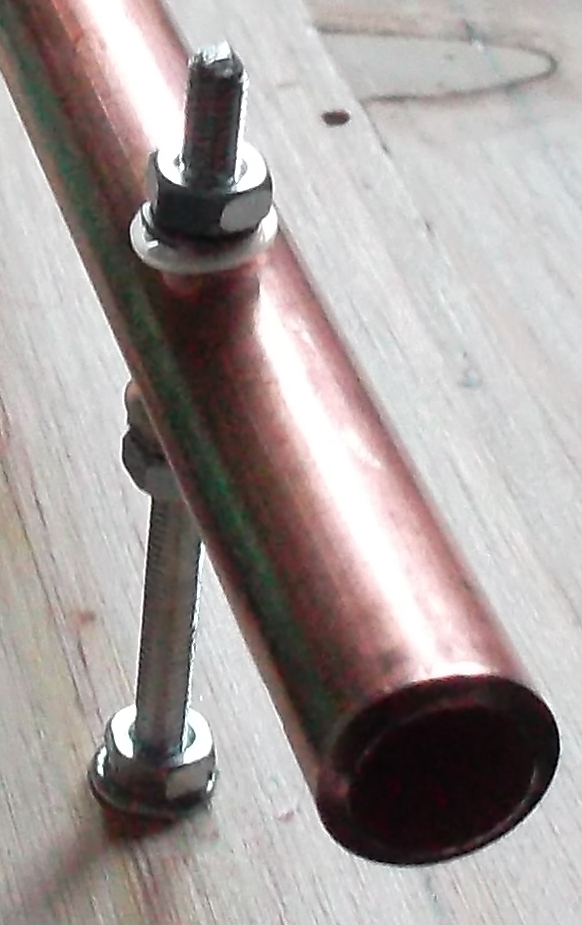
\includegraphics[keepaspectratio=true, width=40mm]{../pics/assembly/mounted_pipe_cropped.jpg}
  \end{tabular}
\end{center}

%%
\newpage
\section{Bill of materials}
\begin{center}
  \begin{tabular}{|c|c|c|c|c|}
    %% titles
    \hline
    \textit{reference} &
    \textit{reseller} &
    \textit{description} &
    \textit{quantity} &
    \textit{price (euros)}\\
    %% copper pipe
    \hline
    copper pipe\\
    \hline
  \end{tabular}
\end{center}

%%
\newpage
\section{References}
\begin{itemize}
\item wiki\_acous\_reson: http://en.wikipedia.org/wiki/Acoustic\_resonance
\item tamhigh\_xylo: staff.tamhigh.org/lapp/xylophone.pdf
\end{itemize}


\end{document}
